\section{Comparison with previous work}

\cite{de2014evolution} simulate the phase of mass transfer for the $\xi$ Tau system using AMUSE. Their study focuses on the effect of the initial mutual inclination on the evolution of the system. Their models include overshooting and they report a type B mass transfer, which is also the case for my models including overshooting. Additionally, they also encounter mass transfer that leads to a common envelope-like structure around the inner binary. Except for the evolution of the inner semi-major axis, the evolution of the outer and inner orbits in my study is qualitatively similar to their results. On the one hand, in \cref{sec:resolution}, I demonstrate that the resolution of my simulations is probably poor, hence this may be a reason behind this discrepancy. On the other hand, \cite{de2014evolution} claim to use the same resolution. Their study covers a larger mass transfer duration, $\sim 40$ yr, but this is expected as in my case the widening of the inner orbit brings the system relatively fast to the unstable regime. In conclusion, my results qualitatively agree with \cite{de2014evolution} study, but higher resolution simulations are needed to confidently conclude about the evolution of the inner semi-major axis during mass transfer.

In my study, I also investigate the importance of the inner binary's accretion efficiency. The lack of theoretical predictions makes the comparison of the results difficult, but some estimations can be made. In \cite{zwart2019triple} study, the formation of a circumbinary disk leads to accretion efficiency up to $\beta \gtrsim 0.8$, while in my study the model with the highest accretion efficiency corresponds to $\beta = 0.53$, see \cref{fig:inclination_binary_eff}. Keep in mind that, the inner binary in their study has nearly the same size, a comparable period, but smaller accretion radii then my binary components. Despite that, the accretion efficiency is $\sim 30\%$ higher. As a result, it appears that, in the absence of a forming disk, the inner binary rotation makes accretion of incoming mass more difficult since part of it gets ejected via a slingshot effect. In conclusion, the accretion efficiency of the inner binary is most likely strongly related to whether or not a circumbinary disk forms. The absence of a forming disk suggests a highly non-conservative mass transfer. This is an intriguing speculation and an interesting topic for future research.

For the maximal accretion case, I find that a value of $\eta \approx 4$ can describe the evolution of the semi-major axis of the outer orbit, while a value of $\eta \approx 7$ is needed to match the minimal accretion case assuming the same amount of mass is lost. The latter results in a shorter timescale for the process, making these systems more difficult to detect. In comparison, a value of $\eta = 6$ is consistent with non-conservative mass transfer in binaries through the second Lagrangian point \citep{flannery1977origin,portegies1995formation} and it is associated with the formation of a circumbinary ring, see \cref{fig:triple_equop}. Additionally, a value of $\eta \gtrsim 3$ is derived in \cite{portegies1995formation} study by matching the orbital evolution and birthrate of Be-type X-ray binaries that experience non-conservative mass transfer. In addition, \cite{de2014evolution, zwart2019triple} 
 also report values of $\eta = 3-4$ in their studies of mass-transferring triples. 

Finally, \cite{zwart2019triple,leigh2020mergers} report that given the formation of a circumbinary disk via \ac{rlof} by the outer star, a preferable accretion towards the less massive binary component occurs. Despite the fact that in my simulations no disk forms, I encounter the same behavior for the models with $i_{mut} \neq 0^{\circ}$, see \cref{fig:inclination_binary_eff}
\begin{figure}[H]
    \centering
    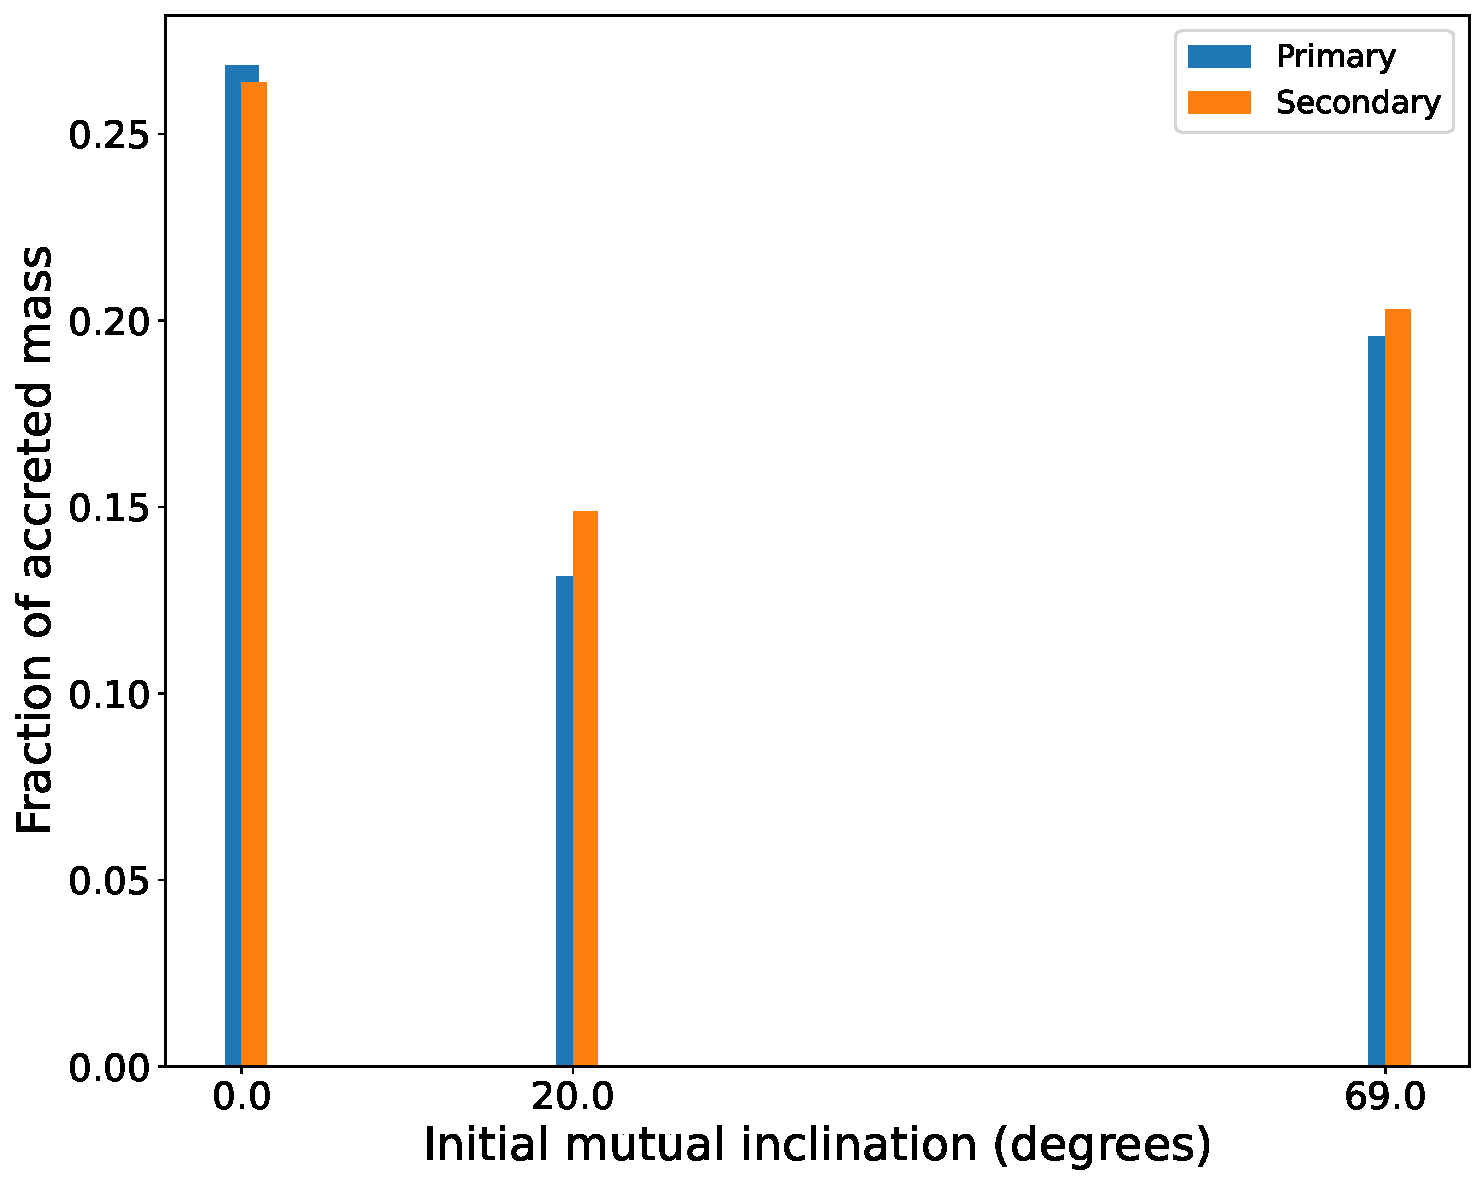
\includegraphics[width=0.9\textwidth]{Thesis/graphs/inclination_case/incliantion_binary_acc_efficiency.pdf}
    \caption{Fraction of the accreted mass by the inner binary stars for different initial inclination of the outer orbit relative to the inner orbit. The secondary star is the initially less massive star of the inner binary system.}
    \label{fig:inclination_binary_eff}
\end{figure}
Quantify distinct trends in \cref{fig:inclination_binary_eff} is not trivial, due to the complicated transport of mass, angular momentum and energy between the outer star, and the accretion stream onto the individual inner stars. More importantly, running higher resolution simulations before trying to interpret this result is necessary. Because gas drag may alter the details of the accretion process. Nonetheless, this outcome is interesting to be investigated due to the fact that it hints towards a mechanism of producing equal mass binaries. 
